\documentclass[12pt,a4paper]{article}

\usepackage[utf8]{inputenc}
\usepackage{graphicx}
\usepackage[spanish]{babel}
\usepackage{float}				%Para poner las imagenes exactamente donde se me cante las pelotas en caso de quererlo, poniendole [H]
\usepackage{amsmath}
\usepackage{epstopdf}
\usepackage{geometry}
\usepackage{hieroglf}
\usepackage{subcaption}
\usepackage[justification=centering]{caption}
\usepackage[colorlinks=true, allcolors=blue]{hyperref}
\geometry{
a4paper,
left=20mm,
right=20mm,
top=25mm,
bottom = 20mm
}
\usepackage{float}
\usepackage{units}
\marginparwidth=2cm
\usepackage[colorinlistoftodos]{todonotes}

% \usepackage{hyperref}   %Esto es para ir a los links

\title{\mathbf{Mecánica de Medios Continuos \\Práctica 3 \\ Descripción de la deformación}}
\author{Universidad de Cuenca}
\begin{document}
\maketitle
\begin{enumerate}
    \item Una manera de visualizar la deformación es mostrar como curvas dibujadas sobre la superficie del cuerpo se ven después de haberse deformado. Dada la configuración inicial de la parte superior de la siguiente figura, determine cuáles de las figuras de la parte inferior corresponden a deformaciones homogéneas.
    \begin{figure}[H]
        \centering
        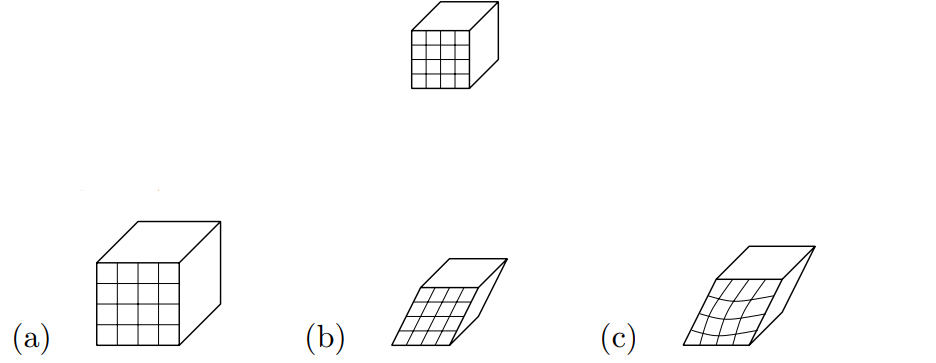
\includegraphics[width=0.8\textwidth]{tp3-1.png}
    
    \end{figure}
    \item Se sabe que el tensor de tensiones de Cauchy para cierto medio continuo
    (un fluido) viene dado por $\boldsymbol{\sigma} = -p\mathbf{I} + \lambda Tr(\mathbf{d})\mathbf{I} + 2\mu\mathbf{d}$, donde \textbf{d} es el
    tensor de velocidad de deformación, p es la presión hidrostática y $\lambda$, $\mu$ son
    constantes. Dado un sistema de coordenadas cartesianas xyz, cuya base
    ortonormal correspondiente es ${\mathbf{e_1, e_2, e_3}}$, considere que el campo de
    velocidades viene dado por $\mathbf{v} = kx\mathbf{e_1} + ky\mathbf{e_2} + kz\mathbf{e_3}$. Tome la constante k
    igual al $(n + 2)-1$, donde n es el  ́último dígito de su número de cédula.
    Calcule la expresión matricial del tensor de Cauchy en la base dada.
    \item Considere un medio continuo cuya ecuación del movimiento es
    \begin{equation}
        \mathbf{x}(\mathbf{X},t)=e^{mt}\mathbf{X}
    \end{equation}
    
    donde m es igual al último dígito de su número de cédula más uno.
    \begin{enumerate}
        \item Encuentre la expresión general del estiramiento.
        \item Encuentre el volumen que tendría para $t=5$ un medio continuo que en la
        configuración de referencia es una esfera de radio 1.
    \end{enumerate}
   \item Considere un medio continuo cuya ecuación del movimiento es
   \begin{equation}
       \mathbf{x}(\mathbf{X},t)=(mt+1)\mathbf{X}
   \end{equation}
   
   donde m es igual al último dígito de su número de cédula más uno.
   \begin{enumerate}
       \item Encuentre la expresión del alargamiento unitario para $t=2$.
       \item Encuentre el volumen que tendría para $t=5$ un medio continuo que en la
       configuración de referencia es una esfera de radio 1.
   \end{enumerate}
\item En un tiempo dado, la ecuación de movimiento de un medio continuo es:
    \begin{equation}
        x_1=X_1,x_2=X_3+4,x_3=X_2
    \end{equation}
    Si la configuración inicial es el cubo B de lado 2 que se muestra en la siguiente figura, dibuje la configuración  actual en el mismo eje de referencia, indiciando qué vertices corresponden al a, b y c.   
    \begin{figure}[H]
        \centering
        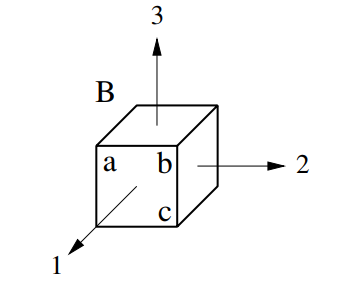
\includegraphics[width=0.4\textwidth]{tp3-2.png}
    \end{figure}
    \item En un tiempo dado, la ecuación de movimiento de un medio continuo es:
    \begin{equation}
        x_1=X_1+/alpha X_2,x_2=X_2,x_3=X_3
    \end{equation}
    \item En un tiempo dado, la ecuación de movimiento de un medio continuo es:
    \begin{equation}
        x_1=X_1+\alpha X_2,x_2=X_2,x_3=X_3,
    \end{equation}
    con $\alpha>0$ constante. Dicha deformación se conoce como \textit{corte simple} en el plano $\mathbf{e_1,e_2}$. Si la configuración inicial es el cubo $B$ de lado 1 que se observa en la siguiente figura (línea punteada), el resultado es el cubo deformado $B'$ (línea continua).    
    \begin{figure}[H]
        \centering
        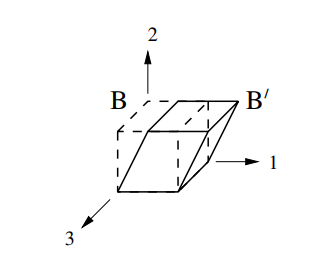
\includegraphics[width=0.4\textwidth]{tp3-3.png}
    \end{figure}
    \begin{enumerate}
        \item Calcular los componentes del tensor de Cauchy-Green.
        \item Encuentre el corte en la dirección $\mathbf{e_1,e_2}$ y en la dirección $\mathbf{e_2,e_3}$. ¿Qué sucede cuando $\alpha\rightarrow\infty$?
        \item Encontrar los valores extremos de el estiramiento $\lambda$ y las direcciones en las que ocurren. ¿Coinciden estas direcciones con alguna de las diagonales $\pm\frac{1}{\sqrt{2}}(\mathbf{e_1+e_2})$ o $\pm\frac{1}{\sqrt{2}}(\mathbf{e_1-e_2})$ del plano $\mathbf{e_1,e_2}$?
\end{enumerate}
\end{document}